

\documentclass{article}

\usepackage{amsmath}
\usepackage{graphicx}


\author{Qing Scholten, Wessel van Sommeren}
\title{Controlling a rabbit plaque}

\begin{document}

\maketitle
\newpage
\tableofcontents
\newpage

\section{Introduction}
For the base case we use the fact that a rabbit on average gets 4 - 8 babies per 60 days. So we take 6 on average that means one rabbit produces 0.1 rabbit per day. A rabbit in the wild live up to 9 nine years this means 0.000312109862672 rabbits die per day per rabbit. This means we get 
$$
\frac{dP(t)}{dt} = 0.1P(t)-000312109862672P(t)
$$

We take $P(0) = 13$ as starting population
\\
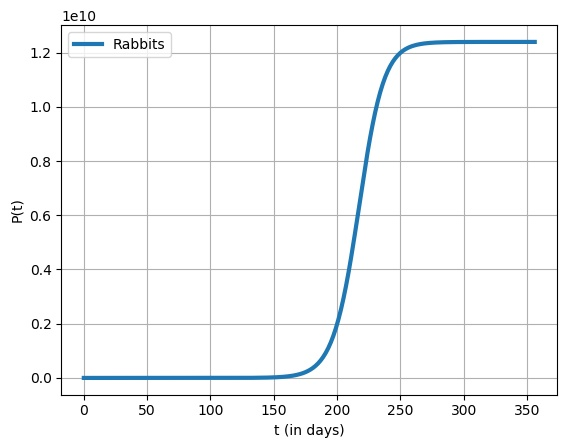
\includegraphics{Pictures/unr_rabbitts}
\end{document}
